\chapter{Introduction}

In this master thesis we implement and discuss the reulst of the propsed model 
for machine teaching. \cite{CNN:deeplearning}

\section{Background}

Lorem ipsum dolor sit amet, cu graecis propriae sea. Eam feugiat docendi an, ei scripta blandit pri. Nonumes delicata reprimique nam ut. Eu suas alterum concludaturque est, ferri mucius sensibus id sed~\cite{raftAlg}.

We can do glossary for acronymes and abriviations also: \gls{saas}. As you see the first time it is used, the full version is used, but the second time we use \gls{saas} the short form is used. It is also a link to the lookup.


\subsection{Listings}
You can do listings, like in Listing~\ref{ListingReference}
\begin{lstlisting}[caption={[Short caption]Look at this cool listing. Find the rest in Appendix~\ref{Listing}},label=ListingReference]
$ java -jar myAwesomeCode.jar
\end{lstlisting}

You can also do language highlighting for instance with Golang:
And in line~\ref{LineThatDoesSomething} of Listing~\ref{ListingGolang} you can see that we can ref to lines in listings.

\begin{lstlisting}[caption={Hello world in Golang},label=ListingGolang,escapechar=|]
package main

import "fmt"

func main() {
    fmt.Println("hello world") |\label{LineThatDoesSomething}|
}

\end{lstlisting}

\subsection{Figures}

Example of a centred figure
\begin{figure}[H]
    \centering
    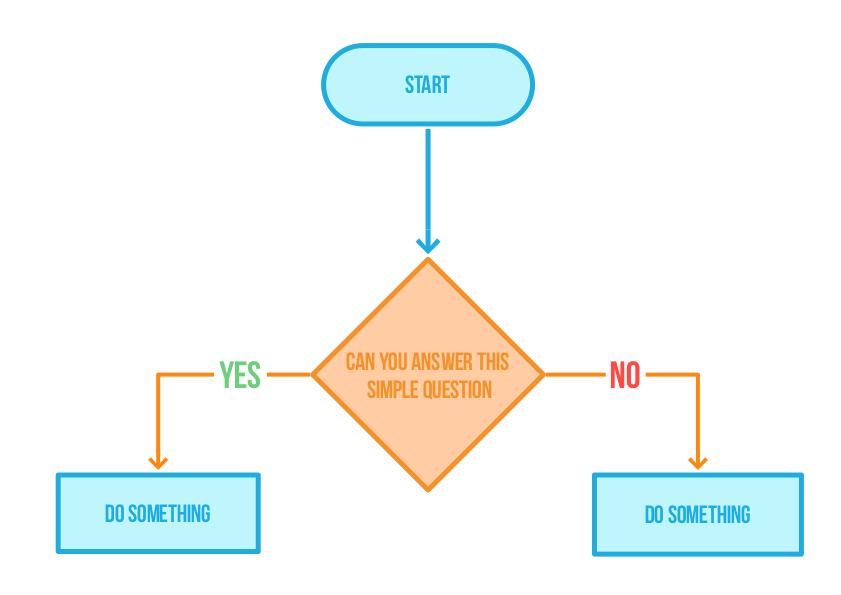
\includegraphics[scale=0.5]{figures/Flowchart}
    \caption{Caption for flowchart}
  	\medskip 
	\hspace*{15pt}\hbox{\scriptsize Credit: Acme company makes everything \url{https://acme.com/}}
    \label{FlowchartFigure}
\end{figure}

\subsection{Tables}

We can also do tables. Protip: use \url{https://www.tablesgenerator.com/} for generating tables.
\begin{table}[H]
\centering
\caption{Caption of table}
\label{TableLabel}
\begin{tabular}{|l|l|l|}
\hline
Title1 & Title2 & Title3 \\ \hline
data1  & data2  & data3  \\ \hline
\end{tabular}
\end{table}

\subsection{\gls{git}}

\gls{git} is fun, use it!